% ============================================================================
% Lecture 18 (B17): PINNs I --- Residual Learning for ODEs and PDEs
% Deep Learning for Solving and Estimating Dynamic Models in Economics and Finance
% Course author: Simon Scheidegger
% ============================================================================

\documentclass[aspectratio=169,11pt]{beamer}

% ---------- Theme and colors ----------
\usecolortheme{dove}
\setbeamertemplate{navigation symbols}{}
\setbeamertemplate{footline}{%
  \hfill\usebeamerfont{page number in head/foot}%
  \usebeamercolor[fg]{normal text}%
  \insertframenumber\,/\,\inserttotalframenumber\kern1em\vskip4pt}
\setbeamerfont{frametitle}{size=\huge}

% ---------- Packages ----------
\usepackage[utf8]{inputenc}
\usepackage[T1]{fontenc}
\usepackage{amsmath,amssymb,amsfonts}
\usepackage{bm}
\usepackage{graphicx}
\usepackage{tikz}
\usetikzlibrary{shapes,arrows.meta,positioning,calc,fit,backgrounds,patterns,decorations.pathreplacing}
\usepackage{pgfplots}
\pgfplotsset{compat=1.18}
\usepackage{booktabs}
\usepackage{hyperref}
\usepackage{multicol}
\usepackage{xcolor}
\usepackage{algorithm}
\usepackage{algorithmic}
\usepackage{listings}

% ---------- Listings style for Python ----------
\lstset{
    language=Python,
    basicstyle=\small\ttfamily,
    keywordstyle=\color{uzhblue}\bfseries,
    commentstyle=\color{uzhgreydark}\itshape,
    stringstyle=\color{darkgreen},
    showstringspaces=false,
    breaklines=true,
    breakatwhitespace=true,
    columns=fullflexible,
    frame=none,
    xleftmargin=0pt,
    aboveskip=4pt,
    belowskip=4pt,
    escapeinside={(*@}{@*)},
}

% ---------- Custom colors ----------
\definecolor{uzhblue}{rgb}{0,0,0.5}
\definecolor{uzhgreylight}{RGB}{236,238,241}
\definecolor{uzhgreydark}{RGB}{81,86,94}
\definecolor{harvardcrimson}{RGB}{153,0,0}
\definecolor{unil@blue}{RGB}{0,140,204}
\definecolor{unil@black}{RGB}{35,31,32}
\definecolor{darkgreen}{RGB}{0,100,0}
\definecolor{darkred}{RGB}{139,0,0}
\definecolor{softblue}{RGB}{70,130,180}
\definecolor{softorange}{RGB}{230,159,0}
\definecolor{softgreen}{RGB}{0,158,115}

% ---------- Set beamer colors ----------
\setbeamercolor{frametitle}{bg=uzhgreylight, fg=uzhblue}
\setbeamercolor{title}{fg=uzhblue}
\setbeamercolor{structure}{fg=uzhblue}
\setbeamercolor{block title}{bg=unil@blue, fg=white}
\setbeamercolor{block body}{bg=uzhgreylight}
\setbeamercolor{block title alerted}{bg=darkred,fg=white}
\setbeamercolor{block body alerted}{bg=red!5}
\setbeamercolor{block title example}{bg=darkgreen,fg=white}
\setbeamercolor{block body example}{bg=green!5}
\setbeamercolor{item}{fg=unil@black}
\setbeamercolor{normal text}{fg=unil@black}

% ---------- Emphasis and hyperlinks ----------
\newcommand{\emphc}[1]{\textcolor{harvardcrimson}{#1}}
\hypersetup{colorlinks,linkcolor=harvardcrimson,urlcolor=harvardcrimson}

% ---------- Math commands ----------
\newcommand{\x}{\bm{x}}
\newcommand{\w}{\bm{w}}
\newcommand{\bb}{\bm{b}}
\newcommand{\z}{\bm{z}}
\newcommand{\W}{\bm{W}}
\newcommand{\X}{\bm{X}}
\renewcommand{\a}{\bm{a}}
\newcommand{\R}{\mathbb{R}}
\newcommand{\E}[1]{\mathbb{E}\!\left[#1\right]}
\DeclareMathOperator*{\argmin}{arg\,min}
\DeclareMathOperator*{\argmax}{arg\,max}

% ---------- Title ----------
\title[Lecture 18 (B17)]{Lecture 18 (B17): Physics-Informed Neural Networks --- Foundations}
\subtitle{DEQN vs PINN, automatic differentiation for PDEs, training pipeline, architecture}
\author{Simon Scheidegger}
\institute{HEC, University of Lausanne}
\date{}
\begin{document}

% Custom command used in some "Finger Exercise" frame titles.
\providecommand{\exercisepause}{%
  \tikz[baseline=(X.base)]{\node[fill=darkgreen!80!black, text=white,
  rounded corners=2pt, inner sep=3pt, font=\scriptsize\bfseries](X){PAUSE};}}

{\setbeamercolor{background canvas}{bg=uzhgreylight}
\begin{frame}
\titlepage
\end{frame}
}

% --- About-this-lecture orientation ---
\begin{frame}{About this lecture}
\small
\begin{block}{What this lecture covers}
\begin{itemize}\itemsep2pt
  \item Discrete-time DEQN vs continuous-time PINN: what changes in the loss
  \item Automatic differentiation for PDEs; collocation points
  \item PINN training pipeline (Adam $\to$ L-BFGS in fp64), network architecture, why tanh
\end{itemize}
\end{block}
\begin{block}{Builds on}
\begin{itemize}\itemsep2pt
  \item Lecture 06 (DEQN loss as residual)
\end{itemize}
\end{block}
\begin{block}{Leads to}
\begin{itemize}\itemsep2pt
  \item Lecture 19 (boundary conditions and economic PDEs: HJB, Black-Scholes)
\end{itemize}
\end{block}
\end{frame}

\begin{frame}{Outline}
\begin{enumerate}
    \item \textbf{From DEQNs to PINNs}\\
    {\small Bridging discrete and continuous time; the PINN loss.}

    \vspace{0.4em}
    \item \textbf{PINN Fundamentals}\\
    {\small Automatic differentiation for PDEs, collocation, training loop.}

    \vspace{0.4em}
    \item \textbf{Soft vs.\ Hard Boundary Conditions}\\
    {\small Trial solutions, 2D Poisson, practical guidance.}

    \vspace{0.4em}
    \item \textbf{Economic Applications: HJB Equation}\\
    {\small Cake-eating problem, scaled trial solution + hard BCs, Adam $\to$ L-BFGS, analytical benchmark; DGM as optional high-D architecture.}

    \vspace{0.4em}
    \item \textbf{Financial Applications: Black--Scholes}\\
    {\small Option pricing via PINNs, comparison with analytical formula.}
\end{enumerate}
\end{frame}

% --- Slide 3: Roadmap ---
\begin{frame}{Roadmap of This Lecture}
\begin{columns}[T]
\column{0.48\textwidth}
\textbf{From DEQNs to PINNs}
\begin{itemize}
    \item Discrete vs.\ continuous time
    \item The PINN loss function
    \item DEQN vs.\ PINN comparison
\end{itemize}

\vspace{0.5em}
\textbf{PINN Fundamentals}
\begin{itemize}
    \item Autograd for PDEs
    \item Collocation and training
    \item Warm-up: 1D ODE example
\end{itemize}

\column{0.48\textwidth}
\textbf{Boundary Conditions}
\begin{itemize}
    \item Soft vs.\ hard enforcement
    \item Trial solutions
    \item 2D Poisson example
\end{itemize}

\vspace{0.5em}
\textbf{Econ \& Finance}
\begin{itemize}
    \item HJB / cake-eating: trial solution + hard BCs
    \item Adam warm-start, L-BFGS polish, FP64
    \item Black--Scholes PDE; DGM as optional architecture
\end{itemize}
\end{columns}
\end{frame}

% ============================================================================
% PART I: FROM DEQNs TO PINNs
% ============================================================================

% --- Slide 4: Section Divider ---
\begin{frame}{}
\vfill
\begin{center}
{\Huge \textcolor{uzhblue}{\textbf{Part I}}}\\[12pt]
{\LARGE From DEQNs to PINNs}
\end{center}
\vfill
\end{frame}

% --- Slide 5: Recall the DEQN Loss ---
\begin{frame}{Recall: The DEQN Loss}
\textbf{Yesterday:} we trained a neural network $\mathcal{N}_\theta$ to satisfy
economic equilibrium conditions in \emphc{discrete time}:
\[
\boxed{
\ell_\theta^{\text{DEQN}} = \frac{1}{N}\sum_{i=1}^{N}
\bigl\|G\bigl(\x_i,\,\mathcal{N}_\theta(\x_i)\bigr)\bigr\|^2
}
\]

\vspace{0.3em}
\begin{itemize}
    \item $G(\cdot) = 0$: Euler equations, budget constraints, market clearing
    \item Training points $\x_i$: simulated from the model's own dynamics
    \item \emphc{No labeled data needed}---structural equations \emph{are} the loss
\end{itemize}

\vspace{0.5em}
\textbf{Today's question:}
What if the economic model is formulated in \emphc{continuous time}?
\end{frame}

% --- Slide 6: Discrete vs Continuous Time ---
\begin{frame}{Discrete vs.\ Continuous Time}
\begin{columns}[T]
\column{0.47\textwidth}
\begin{block}{Discrete Time (DEQN)}
\centering\small
\vspace{0.2em}
Euler equation:\\[4pt]
$u'(c_t) = \beta\,\E{u'(c_{t+1})\,R_{t+1}}$\\[8pt]
State transition:\\[4pt]
$\x_{t+1} = h(\x_t, p(\x_t), \varepsilon_{t+1})$\\[8pt]
Loss: algebraic residual $G(\cdot) = 0$
\vspace{0.2em}
\end{block}

\column{0.47\textwidth}
\begin{exampleblock}{Continuous Time (PINN)}
\centering\small
\vspace{0.2em}
HJB equation:\\[4pt]
$\rho\, V = \max_c \bigl\{u(c) + V_a\,\dot{a}\bigr\}$\\[8pt]
State evolution:\\[4pt]
$\mathrm{d}a = (ra - c)\,\mathrm{d}t + \sigma\,\mathrm{d}W$\\[8pt]
Loss: PDE residual $\mathcal{R}(\cdot) = 0$
\vspace{0.2em}
\end{exampleblock}
\end{columns}

\vspace{0.6em}
\begin{center}
{\small \emphc{Key shift:} from algebraic residuals to \textbf{differential} residuals---we need \emphc{derivatives} of the neural network.}
\end{center}
\end{frame}

% --- Slide 7: Why Continuous Time? ---
\begin{frame}{Why Continuous Time Matters}
\textbf{Many frontier models} are formulated in continuous time:

\vspace{0.3em}
\begin{itemize}
    \item \emphc{Heterogeneous-agent models:} Achdou, Han, Lasry, Lions \& Moll (2022)---income and wealth distribution dynamics via HJB--KFE systems

    \vspace{0.2em}
    \item \emphc{Mean-field games:} optimal policy with a continuum of interacting agents

    \vspace{0.2em}
    \item \emphc{Asset pricing:} Black--Scholes, Heston, jump-diffusion models

    \vspace{0.2em}
    \item \emphc{Macro-finance:} Brunnermeier \& Sannikov (2014), He \& Krishnamurthy (2013)
\end{itemize}

\vspace{0.5em}
\begin{block}{Central bank relevance}
Continuous-time models are the workhorse for \emphc{financial stability analysis}, \emphc{option pricing}, and \emphc{monetary transmission} in modern central banking.
\end{block}
\end{frame}

% --- Slide 8: The PINN Loss ---
\begin{frame}{The PINN Loss Function}
\textbf{Core idea} (Raissi, Perdikaris \& Karniadakis, 2019):

\vspace{0.15em}
Given a PDE $\mathcal{D}[u](\x) = 0$ on domain $\Omega$ with boundary conditions
$\mathcal{B}[u](\x) = 0$ on $\partial\Omega$, define:

\vspace{0.1em}
\[
\boxed{
\ell_\theta^{\mathrm{PINN}} =
\underbrace{\frac{1}{N_r}\sum_{i=1}^{N_r}
\bigl|\mathcal{D}[\mathcal{N}_\theta](\x_i^r)\bigr|^2}_{\text{PDE residual}}
\;+\;
\underbrace{\frac{\lambda}{N_b}\sum_{j=1}^{N_b}
\bigl|\mathcal{B}[\mathcal{N}_\theta](\x_j^b)\bigr|^2}_{\text{boundary/initial conditions}}
}
\]

\vspace{0.05em}
\begin{itemize}
    \item $\mathcal{N}_\theta$: neural network with parameters $\theta$
    \item $\x_i^r$: \emphc{collocation points} in the interior of $\Omega$
    \item $\x_j^b$: points on the boundary $\partial\Omega$
    \item Derivatives $\mathcal{D}[\mathcal{N}_\theta]$ computed via \emphc{automatic differentiation}
\end{itemize}
{\scriptsize \textbf{Warm-up ODE:} for $u''(x)=-1$ on $(0,1)$ with $u(0)=u(1)=0$, use $\mathcal{D}[u]=u''+1$ in the interior and $\mathcal{B}[u]=(u(0),u(1))$ on the boundary.}
\end{frame}

% --- Finger Exercise: PINN Loss ---
\begin{frame}{\exercisepause{} Finger Exercise: Writing a PINN Loss}
\begin{exampleblock}{Exercise}
Consider the ODE $u''(x) = -1$ on $[0,1]$ with boundary conditions $u(0) = u(1) = 0$.
\begin{enumerate}
    \item Write down the PINN residual $\mathcal{R}(x; \theta) = \ldots$ using a neural network $\mathcal{N}(x; \theta)$.
    \item Write the total PINN loss as a sum of a PDE residual term and a boundary term.
    \item What is the exact solution?
\end{enumerate}
\end{exampleblock}
\end{frame}

\begin{frame}{Solution: Writing a PINN Loss}
\begin{block}{Answer}
\begin{enumerate}
    \item $\mathcal{R}(x; \theta) = \frac{\partial^2 \mathcal{N}}{\partial x^2}(x; \theta) + 1$.
    \item $\mathcal{L}(\theta) = \underbrace{\frac{1}{N_r}\sum_{i=1}^{N_r} \bigl|\mathcal{R}(x_i; \theta)\bigr|^2}_{\text{PDE residual}} + \lambda\,\underbrace{\bigl[\mathcal{N}(0;\theta)^2 + \mathcal{N}(1;\theta)^2\bigr]}_{\text{boundary conditions}}$
    \item $u(x) = \tfrac{1}{2}x(1-x)$ satisfies $u''=-1$, $u(0)=u(1)=0$. \checkmark
\end{enumerate}
\end{block}
\end{frame}

% --- Slide 9: DEQN vs PINN Side-by-Side ---
\begin{frame}{DEQN vs.\ PINN: Side-by-Side}
\begin{center}
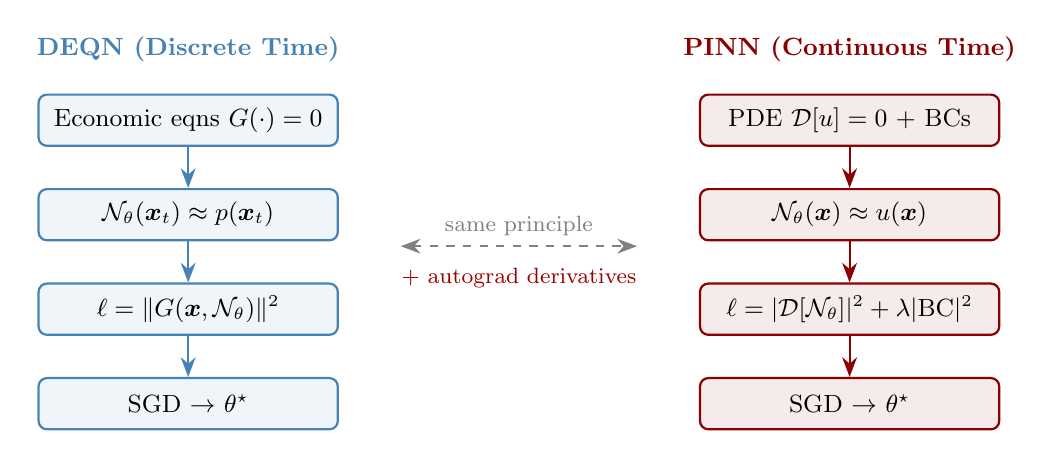
\begin{tikzpicture}[
    deqnbox/.style={rectangle, draw=softblue, thick, fill=softblue!8,
        minimum width=3.8cm, minimum height=0.65cm, font=\small,
        rounded corners=3pt},
    pinnbox/.style={rectangle, draw=darkred, thick, fill=darkred!8,
        minimum width=3.8cm, minimum height=0.65cm, font=\small,
        rounded corners=3pt},
    deqnarr/.style={-{Stealth[length=2.5mm]}, thick, softblue},
    pinnarr/.style={-{Stealth[length=2.5mm]}, thick, darkred}
]
    % DEQN column
    \node[font=\small\bfseries, softblue] at (-4.2,3.5) {DEQN (Discrete Time)};
    \node[deqnbox] (d1) at (-4.2,2.6) {Economic eqns $G(\cdot)=0$};
    \node[deqnbox] (d2) at (-4.2,1.4) {$\mathcal{N}_\theta(\x_t) \approx p(\x_t)$};
    \node[deqnbox] (d3) at (-4.2,0.2) {$\ell = \|G(\x, \mathcal{N}_\theta)\|^2$};
    \node[deqnbox] (d4) at (-4.2,-1.0) {SGD $\to$ $\theta^\star$};
    \draw[deqnarr] (d1) -- (d2);
    \draw[deqnarr] (d2) -- (d3);
    \draw[deqnarr] (d3) -- (d4);

    % PINN column
    \node[font=\small\bfseries, darkred] at (4.2,3.5) {PINN (Continuous Time)};
    \node[pinnbox] (p1) at (4.2,2.6) {PDE $\mathcal{D}[u]=0$ + BCs};
    \node[pinnbox] (p2) at (4.2,1.4) {$\mathcal{N}_\theta(\x) \approx u(\x)$};
    \node[pinnbox] (p3) at (4.2,0.2) {$\ell = |\mathcal{D}[\mathcal{N}_\theta]|^2 + \lambda|\text{BC}|^2$};
    \node[pinnbox] (p4) at (4.2,-1.0) {SGD $\to$ $\theta^\star$};
    \draw[pinnarr] (p1) -- (p2);
    \draw[pinnarr] (p2) -- (p3);
    \draw[pinnarr] (p3) -- (p4);

    % Arrow between
    \draw[dashed, thick, gray, {Stealth[length=2.5mm]}-{Stealth[length=2.5mm]}]
        (-1.5,1.0) -- (1.5,1.0)
        node[midway, above, font=\footnotesize, text=gray] {same principle};
    \node[below, font=\footnotesize, text=gray] at (0,0.85)
        {\emphc{+ autograd derivatives}};
\end{tikzpicture}
\end{center}

\vspace{0.3em}
{\small Both approaches are \emphc{unsupervised}: the physics (economics) \emph{is} the loss function.
The key addition for PINNs: we differentiate the network via \texttt{torch.autograd.grad}.}
\end{frame}

% ============================================================================
% PART II: PINN FUNDAMENTALS
% ============================================================================

% --- Slide 10: Section Divider ---
\begin{frame}{}
\vfill
\begin{center}
{\Huge \textcolor{uzhblue}{\textbf{Part II}}}\\[12pt]
{\LARGE PINN Fundamentals}
\end{center}
\vfill
\end{frame}

% --- Slide 11: Automatic Differentiation ---
\begin{frame}[fragile]{Automatic Differentiation for PDEs}
\textbf{Key tool:} \texttt{torch.autograd.grad} with \texttt{create\_graph=True}.

\vspace{0.4em}
\begin{lstlisting}
# First derivative dy/dx
dydx = torch.autograd.grad(
    y, x,
    grad_outputs=torch.ones_like(y),
    create_graph=True   # keep graph for higher derivs
)[0]
\end{lstlisting}

\vspace{0.3em}
\begin{itemize}
    \item \texttt{create\_graph=True}: retains the computational graph so we can differentiate \emphc{again}
    \item This gives us \emphc{algorithmic} derivatives (up to floating-point precision)---no finite differences!
    \item Works for \emphc{any order}: $\frac{\partial^n}{\partial x^n}$ by chaining $n$ calls
\end{itemize}
\end{frame}

% --- Slide 12: Second Derivatives ---
\begin{frame}[fragile]{Computing Second Derivatives}
\textbf{Chain two autograd calls} to get $y''(x)$:

\vspace{0.3em}
\begin{lstlisting}
# First derivative
dydx = torch.autograd.grad(
    y, x, grad_outputs=torch.ones_like(y),
    create_graph=True)[0]

# Second derivative
d2ydx2 = torch.autograd.grad(
    dydx, x, grad_outputs=torch.ones_like(dydx),
    create_graph=True)[0]
\end{lstlisting}

\vspace{0.3em}
\begin{center}
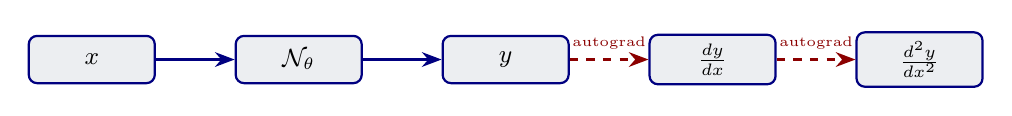
\begin{tikzpicture}[
    mlstep/.style={rectangle, draw=uzhblue, thick, fill=uzhgreylight,
        minimum width=1.6cm, minimum height=0.6cm, font=\small,
        rounded corners=3pt},
    arr/.style={-{Stealth[length=2.5mm]}, thick, uzhblue}
]
    \node[mlstep] (x) {$x$};
    \node[mlstep, right=1.0cm of x] (nn) {$\mathcal{N}_\theta$};
    \node[mlstep, right=1.0cm of nn] (y) {$y$};
    \node[mlstep, right=1.0cm of y] (dy) {$\frac{dy}{dx}$};
    \node[mlstep, right=1.0cm of dy] (d2y) {$\frac{d^2y}{dx^2}$};

    \draw[arr] (x) -- (nn);
    \draw[arr] (nn) -- (y);
    \draw[arr, dashed, darkred] (y) -- (dy) node[midway, above, font=\tiny] {autograd};
    \draw[arr, dashed, darkred] (dy) -- (d2y) node[midway, above, font=\tiny] {autograd};
\end{tikzpicture}
\end{center}
\end{frame}

% --- Slide 13: Collocation Points ---
\begin{frame}[fragile]{Collocation Points}
PINNs evaluate the PDE residual at \emphc{randomly sampled} points---no grid required.

\vspace{0.3em}
\begin{center}
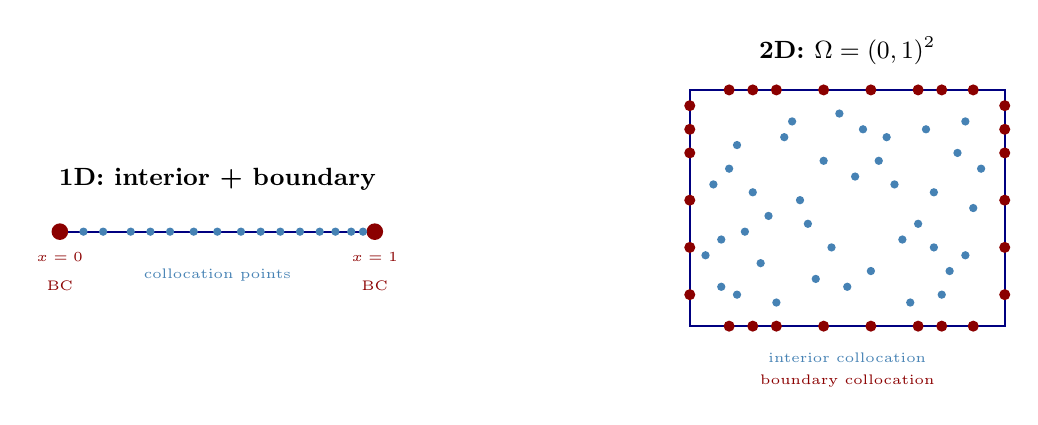
\begin{tikzpicture}
% 1D
\begin{scope}[shift={(-4.5,0)}]
    \draw[thick, uzhblue] (0,0) -- (4,0);
    \fill[darkred] (0,0) circle (3pt) node[below=4pt, font=\tiny] {$x=0$};
    \fill[darkred] (4,0) circle (3pt) node[below=4pt, font=\tiny] {$x=1$};
    \foreach \rx in {0.3,0.55,0.9,1.15,1.4,1.7,2.0,2.3,2.55,2.8,3.05,3.3,3.5,3.7,3.85}{
        \fill[softblue] (\rx,0) circle (1.5pt);
    }
    \node[above, font=\small\bfseries] at (2,0.4) {1D: interior + boundary};
    \node[below=10pt, font=\tiny, softblue] at (2,0) {collocation points};
    \node[below=10pt, font=\tiny, darkred] at (0,-0.15) {BC};
    \node[below=10pt, font=\tiny, darkred] at (4,-0.15) {BC};
\end{scope}

% 2D
\begin{scope}[shift={(3.5,-1.2)}]
    \draw[thick, uzhblue] (0,0) rectangle (4,3);
    % interior points (deterministic pseudo-random)
    \foreach \pt in {
        {0.4,0.5},{1.1,0.3},{2.3,0.7},{3.2,0.4},{0.7,1.2},{1.8,1.0},
        {2.9,1.3},{3.5,0.9},{0.3,1.8},{1.4,1.6},{2.1,1.9},{3.1,1.7},
        {0.6,2.3},{1.7,2.1},{2.5,2.4},{3.4,2.2},{0.9,0.8},{1.3,2.6},
        {2.7,1.1},{3.6,1.5},{0.5,2.0},{1.0,1.4},{2.0,0.5},{3.0,2.5},
        {0.2,0.9},{1.6,0.6},{2.4,2.1},{3.3,0.7},{0.8,1.7},{2.6,1.8},
        {1.2,2.4},{3.7,2.0},{0.4,1.1},{1.9,2.7},{2.8,0.3},{3.5,2.6},
        {0.6,0.4},{1.5,1.3},{2.2,2.5},{3.1,1.0}}{
        \fill[softblue] (\pt) circle (1.5pt);
    }
    % boundary points
    \foreach \rt in {0.5,1.1,1.7,2.3,2.9,3.2,3.6,0.8}{
        \fill[darkred] (\rt,0) circle (2pt);
        \fill[darkred] (\rt,3) circle (2pt);
    }
    \foreach \rt in {0.4,1.0,1.6,2.2,2.5,2.8}{
        \fill[darkred] (0,\rt) circle (2pt);
        \fill[darkred] (4,\rt) circle (2pt);
    }
    \node[above, font=\small\bfseries] at (2,3.2) {2D: $\Omega = (0,1)^2$};
    \node[font=\tiny, softblue] at (2,-0.4) {interior collocation};
    \node[font=\tiny, darkred] at (2,-0.7) {boundary collocation};
\end{scope}
\end{tikzpicture}
\end{center}

\vspace{0.2em}
{\small Points are \emphc{resampled} periodically during training to avoid overfitting to a fixed set.}
\end{frame}

% --- Slide 14: PINN Training Algorithm ---
\begin{frame}{PINN Training Algorithm}
\begin{block}{Algorithm: Physics-Informed Neural Network Training}
\begin{algorithmic}
\footnotesize
\STATE \textbf{Input:} PDE $\mathcal{D}[u]=0$, BCs $\mathcal{B}[u]=0$, network $\mathcal{N}_\theta$, learning rate $\eta$
\FOR{epoch $= 1, \ldots, E$}
    \STATE Sample $N_r$ collocation points $\{\x_i^r\}$ in domain $\Omega$
    \STATE Sample $N_b$ boundary points $\{\x_j^b\}$ on $\partial\Omega$
    \STATE Forward pass: compute $\mathcal{N}_\theta(\x_i^r)$ and $\mathcal{N}_\theta(\x_j^b)$
    \STATE Autograd: compute $\mathcal{D}[\mathcal{N}_\theta](\x_i^r)$ via \texttt{torch.autograd.grad}
    \STATE $\ell_\theta = \frac{1}{N_r}\sum_i |\mathcal{D}[\mathcal{N}_\theta](\x_i^r)|^2 + \frac{\lambda}{N_b}\sum_j |\mathcal{B}[\mathcal{N}_\theta](\x_j^b)|^2$
    \STATE Update: $\theta \leftarrow \theta - \eta\,\nabla_\theta \ell_\theta$
\ENDFOR
\STATE \textbf{Output:} Trained $\mathcal{N}_{\theta^\star}$ approximating the PDE solution
\end{algorithmic}
\end{block}

\vspace{0.2em}
{\small \textbf{Note:} Unlike DEQNs, training points are \emphc{not} simulated from model dynamics---they are drawn uniformly (or adaptively) from the domain.}
\end{frame}

% --- Slide 14b: Optimizer pipeline and FP64 ---
\begin{frame}[shrink=8]{Optimizer Pipeline: Adam $\to$ L-BFGS, in FP64}
\small
\begin{columns}[T]
\column{0.50\textwidth}
\textbf{Two stages.}
\begin{itemize}\itemsep0pt
    \item \emphc{Adam} on resampled collocation: finds a basin.
    \item \emphc{Deterministic L-BFGS} on a \emph{fixed} grid in FP64: closes the residual; resampling per eval breaks the line search.
\end{itemize}

\vspace{0.3em}
\textbf{Why FP64?}
\begin{itemize}\itemsep0pt
    \item $\tanh$-MLP 2nd derivatives lose $\sim$7 digits in FP32.
    \item L-BFGS Wolfe search compares values at exactly that scale.
    \item FP32 plateaus at the noise floor; FP64 keeps shrinking.
\end{itemize}

\column{0.48\textwidth}
\begin{block}{Practical recipe}
\footnotesize
\textbf{1.}~Cast model + data to \texttt{float64}.\\
\textbf{2.}~Adam, lr $10^{-3}$, a few k epochs, resampled collocation.\\
\textbf{3.}~Freeze grid; \texttt{torch.optim.LBFGS} (strong-Wolfe).\\
\textbf{4.}~Stop on residual stagnation.
\end{block}
{\footnotesize Recent precision evidence: \href{https://arxiv.org/abs/2505.10949}{arXiv:2505.10949}.}
\end{columns}

\vspace{0.2em}
{\footnotesize \emphc{Used in notebooks 04, 06, 07, 08:} L-BFGS is the deterministic polish step.  Final residuals remain problem-dependent, so report PDE residuals and solution diagnostics rather than relying on the optimizer label.}
\end{frame}

% --- Slide 15: PINN Architecture ---
\begin{frame}{PINN Architecture}
\begin{center}
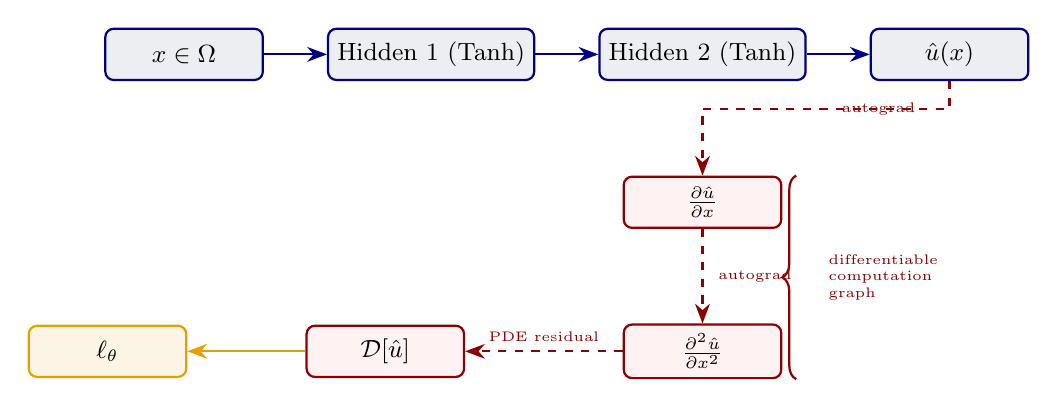
\begin{tikzpicture}[
    mlstep/.style={rectangle, draw=uzhblue, thick, fill=uzhgreylight,
        minimum width=2.0cm, minimum height=0.65cm, font=\small,
        rounded corners=3pt},
    deriv/.style={rectangle, draw=darkred, thick, fill=red!5,
        minimum width=2.0cm, minimum height=0.65cm, font=\small,
        rounded corners=3pt},
    arr/.style={-{Stealth[length=2.5mm]}, thick, uzhblue},
    darr/.style={-{Stealth[length=2.5mm]}, thick, dashed, darkred}
]
    % Main forward path
    \node[mlstep] (in) {$x \in \Omega$};
    \node[mlstep, right=0.8cm of in] (h1) {Hidden 1 (Tanh)};
    \node[mlstep, right=0.8cm of h1] (h2) {Hidden 2 (Tanh)};
    \node[mlstep, right=0.8cm of h2] (out) {$\hat{u}(x)$};

    \draw[arr] (in) -- (h1);
    \draw[arr] (h1) -- (h2);
    \draw[arr] (h2) -- (out);

    % Autograd branch --- shifted left, more vertical spacing
    \node[deriv, below=1.2cm of h2] (du) {$\frac{\partial \hat{u}}{\partial x}$};
    \node[deriv, below=1.2cm of du] (d2u) {$\frac{\partial^2 \hat{u}}{\partial x^2}$};

    \draw[darr] (out.south) -- ++(0,-0.35) -| (du.north)
        node[pos=0.25, right=2pt, font=\tiny] {autograd};
    \draw[darr] (du) -- (d2u) node[midway, right=2pt, font=\tiny] {autograd};

    % PDE residual and loss
    \node[deriv, left=2.0cm of d2u] (res) {$\mathcal{D}[\hat{u}]$};
    \node[rectangle, draw=softorange, thick, fill=softorange!10,
        minimum width=2.0cm, minimum height=0.65cm, font=\small,
        rounded corners=3pt, left=1.5cm of res] (loss) {$\ell_\theta$};

    \draw[darr] (d2u) -- (res) node[midway, above, font=\tiny] {PDE residual};
    \draw[-{Stealth[length=2.5mm]}, thick, softorange] (res) -- (loss);

    % Brace annotation
    \draw[decorate, decoration={brace, amplitude=5pt, mirror}, thick, darkred]
        ([xshift=5pt]du.north east) -- ([xshift=5pt]d2u.south east)
        node[midway, right=8pt, font=\tiny, text=darkred, align=left]
        {differentiable\\computation\\graph};
\end{tikzpicture}
\end{center}

\vspace{0.2em}
{\small The entire pipeline---forward pass \emph{and} derivative computation---is \emphc{differentiable}, enabling end-to-end gradient-based training.}
\end{frame}

% --- Slide 16: Why Tanh? ---
\begin{frame}{Why Tanh Activations for PINNs?}
\begin{columns}[T]
\column{0.55\textwidth}
\textbf{PDE residuals require smooth derivatives.}

\vspace{0.3em}
\begin{itemize}
    \item \emphc{ReLU}: $C^0$ only---second derivative is zero everywhere (useless for $u''$)
    \item \emphc{Tanh}: $C^\infty$---all derivatives are well-defined and informative
    \item \emphc{Softplus}: $C^\infty$, useful for positivity constraints (e.g.\ consumption)
\end{itemize}

\vspace{0.5em}
\begin{alertblock}{Rule of thumb}
For PINNs requiring $k$-th order derivatives, use activations that are at least $C^k$.
\end{alertblock}

\column{0.42\textwidth}
\begin{center}
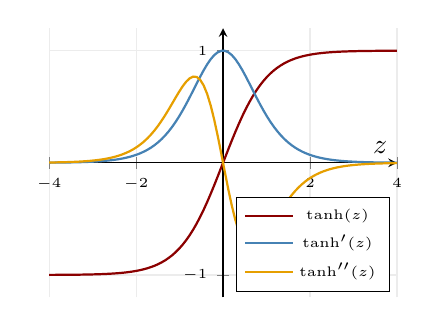
\begin{tikzpicture}
\begin{axis}[
    width=6cm, height=5cm,
    xlabel={$z$}, xlabel style={font=\small},
    tick label style={font=\tiny},
    xmin=-4, xmax=4, ymin=-1.2, ymax=1.2,
    grid=major, grid style={gray!15},
    axis lines=middle,
    legend style={font=\tiny, at={(0.98,0.02)}, anchor=south east},
]
    \addplot[thick, darkred, domain=-4:4, samples=100]{tanh(x)};
    \addlegendentry{$\tanh(z)$}
    \addplot[thick, softblue, domain=-4:4, samples=100]{1 - tanh(x)^2};
    \addlegendentry{$\tanh'(z)$}
    \addplot[thick, softorange, domain=-4:4, samples=100]
        {-2*tanh(x)*(1 - tanh(x)^2)};
    \addlegendentry{$\tanh''(z)$}
\end{axis}
\end{tikzpicture}
\end{center}
\end{columns}
\end{frame}

% --- Slide 17: Warm-up ODE ---
\begin{frame}{Warm-up: Solving an ODE with a PINN}
\textbf{Problem:} $y''(x) = -1$ on $(0,1)$, \; $y(0) = y(1) = 0$.
\quad \textbf{Analytical:} $y(x) = \tfrac{1}{2}x(1-x)$.

\vspace{0.2em}
\begin{columns}[T]
\column{0.45\textwidth}
\textbf{PINN setup:}
\begin{enumerate}\setlength{\itemsep}{1pt}
    \item NN $\mathcal{N}_\theta : [0,1] \to \R$, 2 layers, 20 units
    \item Residual: $r(x) = \mathcal{N}_\theta''(x) + 1$
    \item Loss: PDE residual + BC penalty
\end{enumerate}

\vspace{0.3em}
{\footnotesize
$\ell = \frac{1}{N}\!\sum_i r(x_i)^2 + \mathcal{N}_\theta(0)^2 + \mathcal{N}_\theta(1)^2$
}

\vspace{0.5em}
{\small\textbf{Notebook:} \texttt{01\_ODE\_PINN\_ZeroBCs}}

\column{0.53\textwidth}
\begin{center}
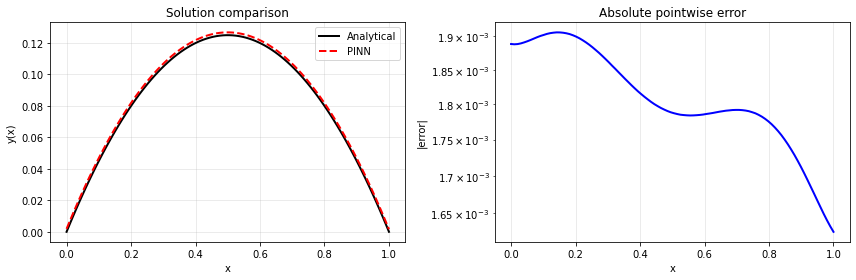
\includegraphics[width=\linewidth]{fig/day6_ext/pinn_ode_warmup.png}\\
{\scriptsize Trained PINN matches analytical solution; pointwise error $\sim 10^{-3}$.}
\end{center}
\end{columns}
\end{frame}

% --- Slide 18: Non-Zero BCs ---
\begin{frame}{Non-Zero Boundary Conditions: The Challenge}
\textbf{Problem:} $y''(x) = -1$ on $(0,1)$ with $y(0) = 1$, $y(1) = 2$.

\vspace{0.2em}
\textbf{Analytical solution:} $y(x) = -\tfrac{1}{2}x^2 + \tfrac{3}{2}x + 1$.

\vspace{0.4em}
\textbf{Soft BC enforcement:}
\[
\ell = \frac{1}{N}\sum_i r(x_i)^2 + \lambda_0\bigl(\mathcal{N}_\theta(0) - 1\bigr)^2 + \lambda_1\bigl(\mathcal{N}_\theta(1) - 2\bigr)^2
\]

\vspace{0.3em}
\textbf{Issues with soft enforcement:}
\begin{itemize}
    \item BCs are only \emphc{approximately} satisfied
    \item Penalty weight $\lambda$ requires \emphc{tuning}: too small $\Rightarrow$ BC violated; too large $\Rightarrow$ PDE ignored
    \item Boundary errors can \emphc{propagate} into the interior
\end{itemize}

\vspace{0.3em}
$\Rightarrow$ \textbf{Motivates hard boundary enforcement} (Part III).
\end{frame}

\end{document}
